% =====================================================================
%  §6 Morse–Smale 复形与 Morse 函数的范畴（6.1–6.3，原文 p36–p41 上半）
%  6.4 起由 ch07 接手
% =====================================================================
\section{Morse--Smale 复形与 Morse 函数的范畴}

\subsection{Morse 理论的记号}

设 $(Y,g_Y)$ 是 $n$ 维紧致定向黎曼流形，$f:Y\to\R$ 是光滑的 Morse 函数（Morse function）。
我们用 $\operatorname{Cr}(f)$ 表示 $f$ 的临界点（critical point）之集。若 $x\in\operatorname{Cr}(f)$，则以 $U_x$
（相应地 $S_x$）表示与 $x$ 相联系的不稳定（相应地稳定）子流形，即
\[
  U_x=\{y\in Y\mid \lim_{t\to+\infty}e^{-t\grad(f)}y=x\},\qquad
  S_x=\{y\in Y\mid \lim_{t\to+\infty}e^{t\grad(f)}y=x\}.
\]

对 $x\in\operatorname{Cr}(f)$，设 $\ind(x)$ 为 $x$ 的 Morse 指标（Morse index），即二次型
$(\partial^2f)|_{T_xY}$ 的负惯性指数。流形 $S_x$ 与 $U_x$ 分别微分同胚于维数为 $\ind(x)$ 与
$n-\ind(x)$ 的开球。由此可知，$S_x$ 的紧支集上同调是一个分次向量空间，其中唯一的
非零一维分量出现在次数 $\ind(x)$ 处：
\[
  H^*_c(S_x)\simeq\Z[-\ind(x)].
\]
生成元的选取定义了 $S_x$ 的一个定向。若函数 $f$ 满足 Morse--Smale 横截性
（transversality）条件，即对任意 $x,y\in\operatorname{Cr}(f)$，流形 $S_x$ 与 $U_y$ 横截相交，则
$Y=\bigsqcup_{x\in\operatorname{Cr}(f)}S_x$ 是 $Y$ 的一个胞腔分解。此时上同调 $H^*(Y,\Z)$ 可以
计算为 Morse 复形 $(M^*(Y,f),\partial)$ 的上同调，其分量为
\[
  M^i(Y,f)=\sum_{x\in\operatorname{Cr}(f),\,\ind(x)=i}H^i_c(S_x).
\]
我们对所有 $x\in\operatorname{Cr}(f)$ 选取流形 $S_x$ 的定向，并赋予 $U_x$ 以对偶定向。分次模
$M^i(Y,f)$ 可以等同于 $\bigoplus_{0\le i\le n}\Z^{Cr_i}[-i]$，其中 $Cr_i$ 是 $f$ 的
指标为 $i$ 的临界点之集。定向的选取给出 $M^*(Y,f)$ 的一组基 $([x])_{x\in\operatorname{Cr}(f)}$。

微分 $\partial$ 是标准的 Morse 微分：
\[
  \partial([x])=\sum_{y\in\operatorname{Cr}(f),\,\ind(y)=\ind(x)+1}
  \deg\bigl((U_x\cap S_y)/\R\bigr)\cdot[y],
\]
其中 $(U_x\cap S_y)/\R$ 是定向的零维流形（带符号的点集），而 $\deg(\cdot)\in\Z$
表示带符号计数的总点数。$\R$ 的作用来自梯度轨道（gradient trajectory）的自然
重参数化 $x\mapsto x+t$。

对平坦向量丛 $\rho$，Morse 复形还有推广 $M^*(Y,f,\rho)$（见 \cite{BZ}、\cite{HL}）。

\begin{yizhu}[扭化的 Morse 复形]
原文到此只给出带平坦向量丛 $\rho$ 的 Morse 复形 $M^*(Y,f,\rho)$ 的记号，未写出其微分，
此处略作说明：$\rho$ 经由沿梯度轨道的和乐进入微分，即把
$\deg((U_x\cap S_y)/\R)$ 换成沿各条连接 $x$ 与 $y$ 的梯度轨道取和乐之迹、再带符号求和。
这正是 \cite{BZ}、\cite{HL} 中的构造；它与下一小节 $\rho_0^*\otimes\rho_1$ 的扭化配套，
使 Morse 范畴的态射空间带有系数。
\end{yizhu}

\subsection{光滑函数的 Morse $A_\infty$-范畴}

这里我们仿照 \cite{FuO} 定义光滑函数的 Morse 范畴 $\mathcal{M}(Y)$。它是 $\C$ 上的
一个 $A_\infty$-预范畴。$\mathcal{M}(Y)$ 的对象是二元组 $(f,\rho)$，其中 $f:Y\to\R$
是光滑函数，$\rho$ 是 $Y$ 上有限维复向量空间的局部系（local system）。在定义对象的
横截性之前，我们先定义函数的横截性。

设给定一列光滑函数 $(f_0,\dots,f_k)$，$k\ge2$，使得所有 $f_i-f_j$（$i\ne j$）都是
Morse 函数；又给定一列临界点 $x_i\in\operatorname{Cr}(f_i-f_{i+1})$（$0\le i\le k-1$）与
$x_k\in\operatorname{Cr}(f_0-f_k)$。我们将用定向二元平面树（oriented binary planar tree）来描述
与这样的序列相关联的某些模空间。固定一棵带 $k+1$ 个尾顶点（tail vertex）的平面三价树
（planar trivalent tree）$T$。在这些尾顶点中取定一个，称为根顶点（root vertex）。我们
把 $T$ 的边沿通往根的最短路径定向。于是 $T$ 成为一棵二元树，并被看作定向树。我们把
$T$ 画在标准单位圆盘 $D\subset\R^2$ 内，使 $T$ 的尾顶点落在 $\partial D$ 上，并使
$D\setminus T$ 的连通分支按顺时针方向从 $0$ 到 $k$ 循环编号。我们约定与根顶点相邻的
两个区域所标的编号为 $0$ 与 $k$。

\begin{center}
  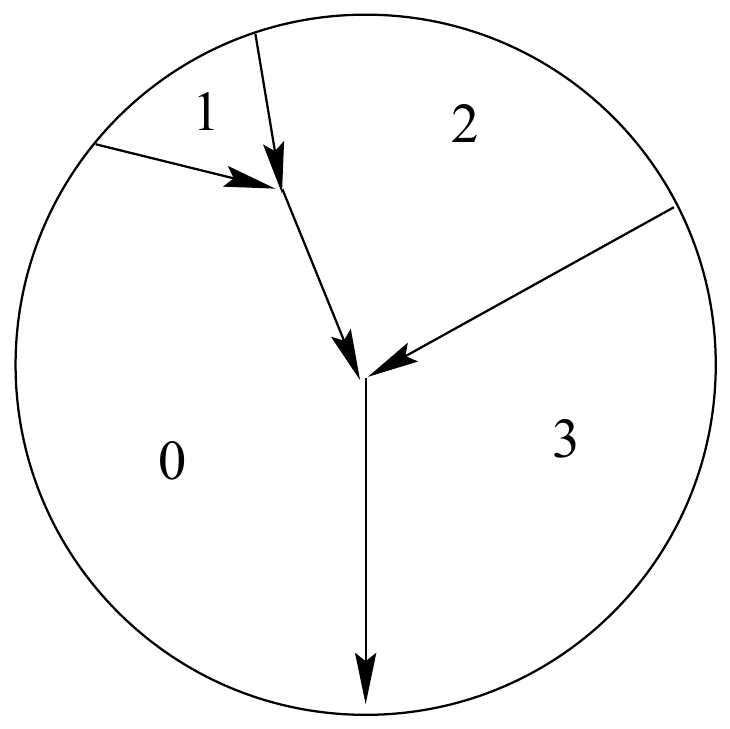
\includegraphics[width=3.09 cm]{figures/fig6_p37_disc_tree}
\end{center}

所谓 $T$ 到 $Y$ 的梯度浸入（gradient immersion），是指连续映射 $j:T\to Y$，满足：

1) 限制 $j|_e$ 把边 $e$ 保向同胚到 $f_{l(e)}-f_{r(e)}$ 的某条梯度线（gradient line）
上的一段区间，其中标号 $l(e)$（相应地 $r(e)$）对应 $D\setminus T$ 中位于 $e$ 左侧
（相应地右侧）的区域。

2) 每个尾顶点 $v$ 映到点 $x_v\in\operatorname{Cr}(f_{l_v}-f_{r_v})$，其中 $l_v$（相应地 $r_v$）
是包含 $v$ 的那条唯一尾边左侧（相应地右侧）区域的标号。

为了在 Morse $A_\infty$-预范畴中定义复合与横截序列，我们需要浸入的二元树（我们称之为
梯度树（gradient tree））。这些结构可以用某些簇（varieties）来刻画，下面就来描述。

设给定如上的一列函数 $(f_0,\dots,f_k)$（$k\ge2$）、一列临界点 $(x_0,\dots,x_k)$，
以及一棵二元平面树 $T$。考虑流形 $Y(T)=Y^{V_i(T)}$，其中 $V_i(T)$ 是 $T$ 的内部顶点
（internal vertex）之集。我们要在 $Y(T)$ 中定义若干子流形。对每个尾顶点 $v_m$，
$0\le m\le k-1$，定义 $Z_{v_m}=\pi_{\hat v_m}^{-1}(U_{x_m})$；对 $m=k$ 定义
$Z_{v_k}=\pi_{\hat v_k}^{-1}(S_{x_k})$。这里 $\hat v_l$ 表示 $T$ 中含 $v_l$ 的那条边的
另一个端点，而 $\pi_v:Y(T)\to Y$ 是对应于 $v\in V_i(T)$ 的那个因子的标准投影。

对每一对 $(f_i,f_j)$，定义子集 $Z_{i,j}\subset Y\times Y$，它由满足 $y_1\ne y_2$ 且
对某个 $t>0$ 有 $y_2=e^{t\grad(f_i-f_j)}y_1$ 的数对 $(y_1,y_2)$ 组成。于是 $Z_{i,j}$
是 $Y\times Y$ 的非紧子流形。

若 $T$ 的一条边的两个端点都是内部顶点，就称它为内边（internal edge）。内边的集合记为
$E_i(T)$。每条内边 $e\in E_i(T)$ 分隔开标号为 $l(e)$（左）与 $r(e)$（右）的两个区域；
对此定义子流形 $Z_e=\pi_e^{-1}(Z_{l(e),r(e)})$，其中 $\pi_e:Y(T)\to Y\times Y$ 是
自然投影。

由定义可知，如上给定的 $T$ 的梯度浸入空间（模去保持尾顶点的同胚）可以等同于
\[
  \mathcal{M}(T;f_0,\dots,f_k;x_0,\dots,x_k):=
  \Bigl(\bigcap_{0\le m\le k}Z_{v_m}\Bigr)\cap\Bigl(\bigcap_{e\in E_i(T)}Z_e\Bigr)
  \subset Y^{V_i(T)}.
\]

\begin{dfn}
称序列 $(f_0,\dots,f_k)$（$k\ge2$）对给定的树 $T$ 是 $T$-横截的，若对任意满足
\[
  \sum_{i=0}^{k-1}\ind(x_i)-\ind(x_k)\le k-2
\]
的交点序列 $(x_0,\dots,x_k)$，子流形族
$\bigl((Z_{v_m})_{0\le m\le k},(Z_e)_{e\in E_i(T)}\bigr)$ 在 $Y(T)$ 中横截（即其中
任意子族之交均横截）。当 $k=1$ 时，称 $(f_0,f_1)$ 是 $T$-横截的（此时 $T$ 只有一种），
若 $f_0-f_1$ 是 Morse 函数且满足 Morse--Smale 横截性条件。
\end{dfn}

\begin{rmk}
与 Fukaya 范畴的情形一样，这里只考虑（虚）维数小于或等于零的空间
\[
  \mathcal{M}(T;f_0,\dots,f_k;x_0,\dots,x_k).
\]
在维数严格为负的情形，我们的条件意味着该模空间为空。
\end{rmk}

可以证明（见 \cite{Fu1}）：在 $(C^\infty(Y))^{\Z}$ 中存在一个第二纲（Baire 纲）的子集，
使得对该集合中任一元素 $(f_i)_{i\in\Z}$、任一严格递增的整数列 $i_0<\dots<i_k$ 以及任一
带 $k+1$ 条尾的平面树 $T$，序列 $(f_{i_0},\dots,f_{i_k})$ 都是 $T$-横截的。

\begin{yizhu}[第二纲集]
第二纲集即补集为第一纲集的子集（原文作 subset of second Baire category）。在
$(C^\infty(Y))^{\Z}$ 这样的完备度量空间中，第二纲集是稠密的，故上述命题是说：对通有的
（generic）函数族，所有横截性条件同时成立。这是本小节一切构造——尤其是下面 $m_k$ 的定义
——得以进行的前提。
\end{yizhu}

\begin{dfn}
若对任意 $m\ge1$、任意带 $m+1$ 条尾的二元树 $T$，任意子序列 $(f_{i_0},\dots,f_{i_m})$
（$i_0<\dots<i_m$）都是 $T$-横截的，则称对象序列 $(f_0,\rho_0),\dots,(f_k,\rho_k)$ 是
横截的。
\end{dfn}

对任意两个横截对象 $W_0=(f_0,\rho_0)$ 与 $W_1=(f_1,\rho_1)$，我们把态射空间
$\Hom_{\mathcal{M}(Y)}(W_0,W_1)$ 定义为 Morse 复形
$M^*(Y,f_0-f_1,\rho_0^*\otimes\rho_1)$。现在来定义 $\mathcal{M}(Y)$ 上的
$A_\infty$-结构。

映射 $m_1:\Hom((f_0,\rho_0),(f_1,\rho_1))\to\Hom((f_0,\rho_0),(f_1,\rho_1))[1]$ 是
Morse--Smale 复形中的标准微分。对横截的对象序列，$k\ge2$ 的高阶复合 $m_k$ 是线性映射
\[
  m_k:\bigotimes_{0\le i\le k-1}\Hom((f_i,\rho_i),(f_{i+1},\rho_{i+1}))
  \longrightarrow\Hom((f_0,\rho_0),(f_k,\rho_k))[2-k].
\]
每个 $m_k$ 都定义为和 $m_k=\sum\pm m_{k,T}$，其中 $T$ 取遍带 $(k+1)$ 条尾的定向二元
平面树的同构类。下面描述这些被加项 $m_{k,T}$。为简单起见，我们只在所有局部系都是秩一的
平凡局部系的情形给出公式。

\begin{yizhu}[$m_{k,T}$ 的符号]
原文对每个被加项只写 $\pm$，未把符号写定：$m_{k,T}$ 的符号由树的平面定向与 §4 的
Koszul 符号约定共同决定。译文照原文保留 $\pm$；读者若要复算，应按该节的符号约定逐顶点
计算。
\end{yizhu}

我们固定临界点 $y_i\in\operatorname{Cr}(f_i-f_{i+1})$（$0\le i\le k-1$）与 $y_k\in\operatorname{Cr}(f_0-f_k)$，
使
\[
  \sum_{0\le i\le k-1}\ind(y_i)=\ind(y_k)+2-k,
\]
并固定流形 $S_{x_i}$（$0\le i\le k$）的定向。由横截序列的定义可知，梯度树的模空间
\[
  \mathcal{M}(T;f_0,\dots,f_k;y_0,\dots,y_k)
\]
是一个定向的紧零维流形。

\begin{yizhu}[原文的一处笔误]
上面刚固定的是临界点 $y_0,\dots,y_k$，故所选定向的流形应为 $S_{y_i}$；原文此处写作
$S_{x_i}$，其中 $x_i$ 是前文定义 $T$-横截性时所用的交点记号。译文照原文译出，此处
按数学意义应读作 $S_{y_i}$。
\end{yizhu}

\begin{dfn}
对 $k\ge2$，用下述公式定义复合 $m_k$：
\[
  m_k([y_0],\dots,[y_{k-1}])=\sum_{[T]}\ \sum_{y_k\in\operatorname{Cr}(f_0-f_k)}
  \deg\bigl(\mathcal{M}(T;f_0,\dots,f_k;y_0,\dots,y_k)\bigr)\cdot[y_k],
\]
其中 $[T]$ 是 $T$ 作为抽象定向平面树的等价类，而 $\deg(\cdot)\in\Z$ 一如既往表示带符号
计数的总点数。
\end{dfn}

对更高秩的局部系，处理方式与 Fukaya 范畴的情形相同：用平坦联络来定义局部系和乐
（holonomy）的类比物。

按下述方式可以得到 $m_k$ 的略有不同的公式。对任意点
$\gamma\in\mathcal{M}(T;f_0,\dots,f_k;y_0,\dots,y_k)$，定义权重（weight）
\[
  w_\gamma=\exp\Bigl(-\frac{1}{\eps}\sum_{e\in E(T)}
  \operatorname{var}_\gamma\bigl(f_{l(e)}-f_{r(e)}\bigr)\Bigr)\in\C_{\eps}.
\]
这里 $\operatorname{var}_\gamma(f_{l(e)}-f_{r(e)})>0$ 是 $f_{l(e)}-f_{r(e)}$ 沿梯度线
$\gamma(e)$ 的变差，其定义如下：
\[
  \operatorname{var}_\gamma\bigl(f_{l(e)}-f_{r(e)}\bigr)
  =(f_{l(e)}-f_{r(e)})(y_{\max})-(f_{l(e)}-f_{r(e)})(y_{\min}),
\]
其中 $y_{\max}$ 与 $y_{\min}$ 是 $\gamma(e)$ 的端点，取法使
$(f_{l(e)}-f_{r(e)})(y_{\max})-(f_{l(e)}-f_{r(e)})(y_{\min})>0$。把标量扩张到
$\C_{\eps}$ 之后，可以在 $\Hom_{\mathcal{M}(Y)}(W_0,W_1)$ 中另取一组基，即对
$y\in\operatorname{Cr}(f_0-f_1)$ 令
\[
  [y]_{\mathrm{new}}=[y]\exp\Bigl(\frac{f_0(y)-f_1(y)}{\eps}\Bigr).
\]
于是 $m_k$ 的公式将有所改变：每条 $\gamma$ 的贡献都要乘以 $w_\gamma$。所得公式与
Fukaya--Oh 范畴的公式类似（见 §5.2）。

\begin{yizhu}[权重 $w_\gamma$ 的来源]
换基 $[y]_{\mathrm{new}}=[y]\exp\bigl((f_0(y)-f_1(y))/\eps\bigr)$ 相当于在每个临界点处
给基向量乘上一个含 $\eps$ 的因子；沿一棵梯度树从尾顶点走到根，这些因子按
$f_{l(e)}-f_{r(e)}$ 逐边相消，只剩每条边上的变差，故整棵树的贡献恰好乘上
$w_\gamma$。这一步与 \cite{FuO} 中用平坦联络的和乐给每条梯度轨道加权是同一回事，也正是
下文把 Morse 侧与 de Rham 侧作比较时 $\eps$ 的着落之处。
\end{yizhu}

\subsection{光滑函数的 de Rham $A_\infty$-范畴}

我们关心的另一个 $A_\infty$-预范畴将是一个微分分次范畴（differential-graded category，
简称 dg-范畴）。换言之，它是一个具有严格单位态射、且 $n\ge3$ 的复合 $m_n$ 全为零的
$A_\infty$-范畴。我们称它为 $Y$ 的 de Rham 范畴（de Rham category），记作 $\DR(Y)$。
$\DR(Y)$ 的对象与 $\mathcal{M}(Y)$ 的相同，即二元组 $(f,\rho)$，其中 $f:Y\to\R$ 是
光滑函数，$\rho$ 是 $Y$ 上的局部系。态射是复形，其公式为
\[
  \Hom_{\DR(Y)}((f_0,\rho_0),(f_1,\rho_1))
  =\Gamma(Y,\wedge^*T_Y^*\otimes\Hom(\rho_0,\rho_1))
\]
注意态射空间不依赖于 $f_0$ 与 $f_1$。态射的复合按显然的方式定义：在 $\rho_0$ 与
$\rho_1$ 的局部平凡化下，它由系数在 $\Omega^*(Y)$ 中的矩阵的乘积给出。

现在可以陈述本节的主要结果了。

\begin{thm}
$A_\infty$-预范畴 $\mathcal{M}(Y)$ 与 $\DR(Y)$ 等价。
\end{thm}

定理的证明将占去本节余下的篇幅。我们先讨论同调扰动理论（homological perturbation
theory）中一组公式的某个版本（见 \cite{GS}、\cite{Me}），它们将给出微分分次代数的
子复形上的 $A_\infty$-结构。然后我们讨论基于 \cite{HL} 中想法的一条证明进路。看起来，
在 Witten 复形的框架内、使用 \cite{BZ} 的方法，可以得到另一个证明（但大概会困难得多）。

% [原文 p36–p41 上半]
